\documentclass[12pt]{article}

%%%%%%%%%%%%%%%%%%%%%%%%%%%%
%%%%%%%%%%%%%%%%%%%%%%%%%%%%
% Load in packages
\usepackage{amsmath}
\usepackage{float}
\usepackage{amssymb}
\usepackage{hyperref}
\usepackage{graphicx}
\usepackage{enumitem}
\usepackage{pgfplots}
\usepackage[top=1in, bottom=1in, left=1in, right=1in]{geometry}

%%%%%%%%%%%%%%%%%%%%%%%%%%%%
%%%%%%%%%%%%%%%%%%%%%%%%%%%%

\begin{document}

\begin{center}
\Large Chapter 21 \& 13 Practice Problems

\medskip

\normalsize Elements of Microeconomics (discussion section 4)

\medskip

\small Jamie Hyder
\end{center}

\section*{Question 1}
A consumer would like to purchase pasta and wine. They have \$100 to spend, pasta costs \$20 per plate and wine costs \$10 per glass.
\begin{enumerate}
    \item How much of each good could they possibly consume?
    \item What is the equation for their budget constraint?
    \item What does their budget constraint look like graphically?
    \item What happens if the price of pasta decreases to \$10?
    \item What happens if income increases to \$160?
\end{enumerate}

\textbf{Answer:} 
\begin{enumerate}
    \item They could consume a maximum of 5 plates of pasta (and 0 glasses of wine) or 10 glasses of wine (and 0 plates of pasta)
    \item Budget constraint: \[100 = 20P + 10W\]
    Where $P$ is number of pasta plates and $W$ is number of glasses of wine.
    \item Graph of budget constraint:
    
    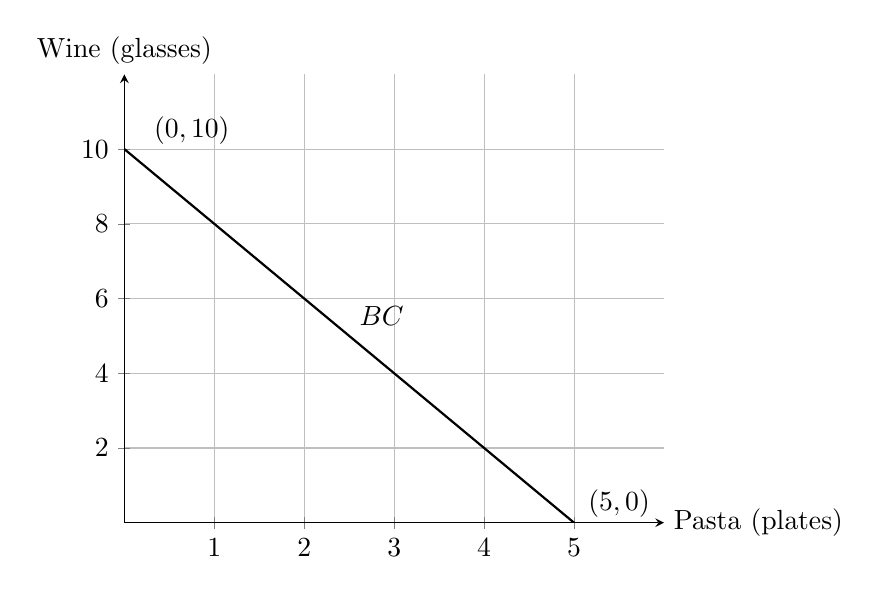
\begin{tikzpicture}
\begin{axis}[
    axis lines=middle,
    xlabel={Pasta (plates)},
    ylabel={Wine (glasses)},
    xmin=0, xmax=6,
    ymin=0, ymax=12,
    xtick={0,1,2,3,4,5},
    ytick={0,2,4,6,8,10},
    grid=both,
    every axis x label/.style={at={(current axis.right of origin)}, anchor=west},
    every axis y label/.style={at={(current axis.above origin)}, anchor=south}
]

% Budget Line: 20P + 10W = 100 → W = 10 - 2P
\addplot[thick] coordinates {(0,10) (5,0)} node[pos=0.5, above right] {$BC$};

% Label intercepts
\node at (axis cs:.75,10.5) {$(0,10)$};
\node at (axis cs:5.5,0.5) {$(5,0)$};

\end{axis}
\end{tikzpicture}

\item Now they can consume a maximum of 10 plates of pasta or 10 glasses of wine. Their new budget constraint is \(100 = 10P + 10W\) and this graphically represented as follows:

 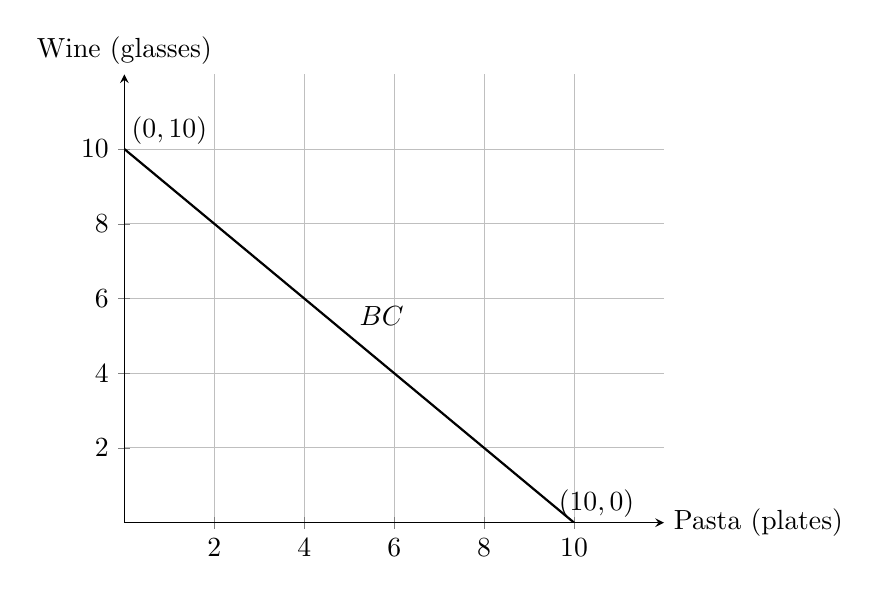
\begin{tikzpicture}
\begin{axis}[
    axis lines=middle,
    xlabel={Pasta (plates)},
    ylabel={Wine (glasses)},
    xmin=0, xmax=12,
    ymin=0, ymax=12,
    xtick={0,2,4,6,8,10},
    ytick={0,2,4,6,8,10},
    grid=both,
    every axis x label/.style={at={(current axis.right of origin)}, anchor=west},
    every axis y label/.style={at={(current axis.above origin)}, anchor=south}
]

% Budget Line: 20P + 10W = 100 → W = 10 - 2P
\addplot[thick] coordinates {(0,10) (10,0)} node[pos=0.5, above right] {$BC$};

% Label intercepts
\node at (axis cs:1,10.5) {$(0,10)$};
\node at (axis cs:10.5,0.5) {$(10,0)$};

\end{axis}
\end{tikzpicture}

\item Now (assuming the original prices) they can consume a maximum of 8 plates of pasta or 16 glasses of wine. The new budget constraint is \(160 = 20P + 10W\). This is represented graphically as follows:

 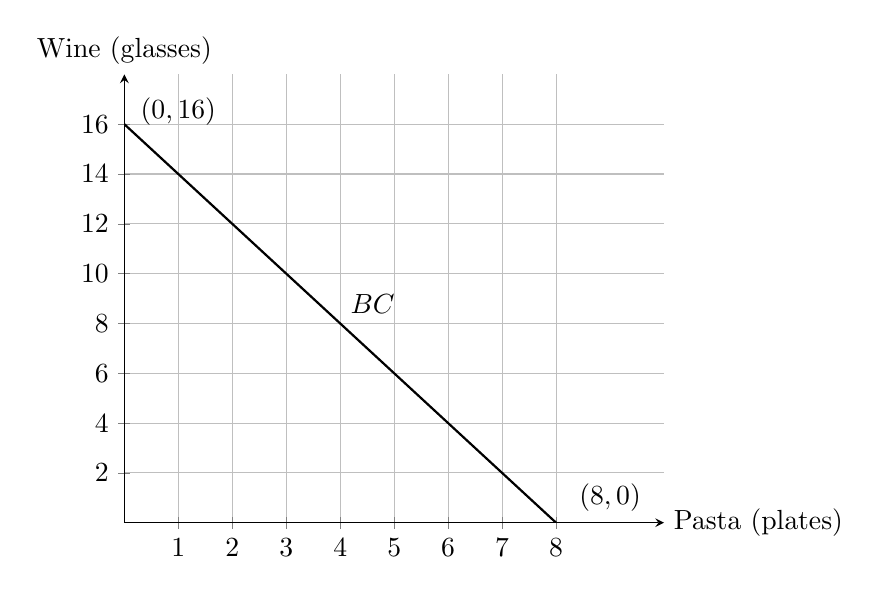
\begin{tikzpicture}
\begin{axis}[
    axis lines=middle,
    xlabel={Pasta (plates)},
    ylabel={Wine (glasses)},
    xmin=0, xmax=10,
    ymin=0, ymax=18,
    xtick={0,1,2,3,4,5,6,7,8},
    ytick={0,2,4,6,8,10,12,14,16},
    grid=both,
    every axis x label/.style={at={(current axis.right of origin)}, anchor=west},
    every axis y label/.style={at={(current axis.above origin)}, anchor=south}
]

% Budget Line: 20P + 10W = 100 → W = 10 - 2P
\addplot[thick] coordinates {(0,16) (8,0)} node[pos=0.5, above right] {$BC$};

% Label intercepts
\node at (axis cs:1,16.5) {$(0,16)$};
\node at (axis cs:9,1) {$(8,0)$};

\end{axis}
\end{tikzpicture}

\end{enumerate}

\newpage
\section*{Question 2}
Using the set up from question 1:
\begin{enumerate}
    \item Draw the indifference curve which represents the maximum satisfaction the consumer could possibly have given their initial budget constraint.
    \item Now consider the increase in income to \$160. Draw the new indifference curve which represents the maximum satisfaction the consumer could possibly have given this budget constraint.
    \item Now consider the decrease in price of pasta to \$10. Draw the new indifference curve which represents the maximum satisfaction the consumer could possibly have given this budget constraint AND illustrate the income and substitution effects as a result of the change. 
\end{enumerate}

\textbf{Answer:}
\begin{enumerate}
    \item Graph with indifference curve:

    \begin{tikzpicture}
\begin{axis}[
    axis lines=middle,
    xlabel={Pasta (plates)},
    ylabel={Wine (glasses)},
    xmin=0, xmax=6,
    ymin=0, ymax=12,
    xtick={0,1,2,3,4,5},
    ytick={0,2,4,6,8,10},
    grid=both,
    every axis x label/.style={at={(current axis.right of origin)}, anchor=west},
    every axis y label/.style={at={(current axis.above origin)}, anchor=south}
]

% --- Budget Line: 20P + 10W = 100 => W = 10 - 2P
\addplot[thick] coordinates {(0,10) (5,0)} node[pos=0.55, above right] ;

% --- Tangency point (optimal bundle) computed from Cobb-Douglas with a=0.4:
% x* = a I / p_x = 0.4*100/20 = 2
% y* = (1-a) I / p_y = 0.6*100/10 = 6
\addplot[only marks, mark=*] coordinates {(2,6)};
\node at (axis cs:2.5,6.6) {Optimal};

% --- Indifference Curve through (2,6):
% Cobb–Douglas U = x^a y^{1-a}, with a=0.4.
% Rearranged: y = K * x^{-a/(1-a)} = K * x^{-2/3}.
% Choose K so that (2,6) lies on the curve: K = 6 * 2^{2/3}.
\addplot[
    thick,
    domain=0.3:5,
    samples=200
] {(6*pow(2,2/3)) * pow(x,-2/3)};
\node at (axis cs:3.7,7.4);

% --- Labels for intercepts
\node at (axis cs:.6,10.2) {$(0,10)$};
\node at (axis cs:5,.5) {$(5,0)$};

% (Optional) show local tangent slope = -2 at the optimum:
\addplot[dashed, domain=1:3] {6 - 2*(x-2)};

\end{axis}
\end{tikzpicture}






\item Now with the increased income:

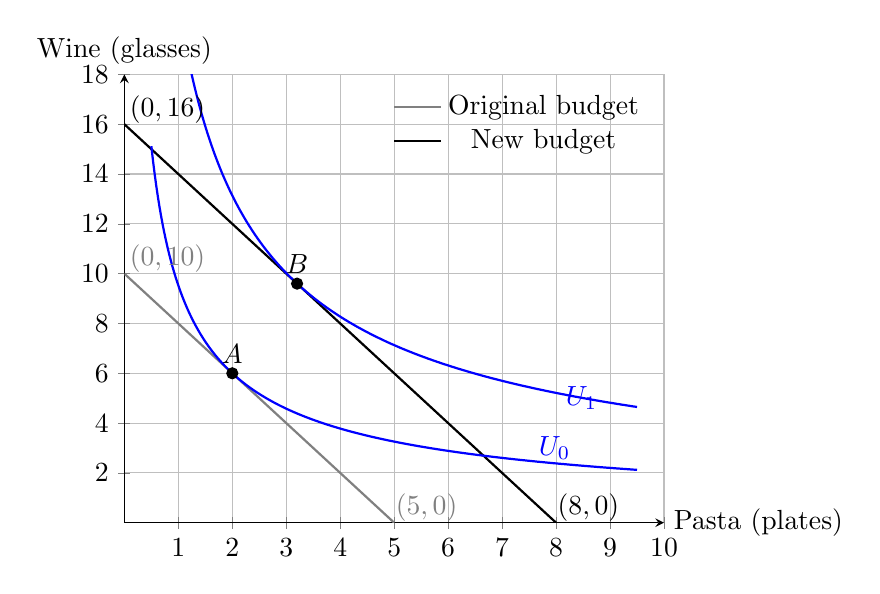
\begin{tikzpicture}
\begin{axis}[
    axis lines=middle,
    xlabel={Pasta (plates)},
    ylabel={Wine (glasses)},
    xmin=0, xmax=10,
    ymin=0, ymax=18,
    xtick={0,1,2,3,4,5,6,7,8,9,10},
    ytick={0,2,4,6,8,10,12,14,16,18},
    grid=both,
    legend style={at={(0.98,0.98)},anchor=north east,draw=none,fill=none},
    every axis x label/.style={at={(current axis.right of origin)}, anchor=west},
    every axis y label/.style={at={(current axis.above origin)}, anchor=south}
]

% ---------- Budget Lines ----------
% Original budget (I=100, p_P=20, p_W=10): slope -2
\addplot[thick, gray] coordinates {(0,10) (5,0)};
\addlegendentry{Original budget}

% New budget (higher income, same prices): slope -2
\addplot[thick, black] coordinates {(0,16) (8,0)};
\addlegendentry{New budget}

% ---------- Optima (Cobb–Douglas with a=0.4) ----------
% A: Initial optimum
\addplot[only marks, mark=*, mark size=2pt] coordinates {(2,6)};
\node[anchor=south] at (axis cs:2,6) {$A$};

% C: New optimum (income scaled 1.6× → bundle scales 1.6×)
\addplot[only marks, mark=*, mark size=2pt] coordinates {(3.2,9.6)};
\node[anchor=south] at (axis cs:3.2,9.6) {$B$};

% ---------- Indifference Curves ----------
% U0 through A=(2,6): y = K0 * x^{-2/3},  K0 = 6 * 2^{2/3} ≈ 9.5244
\addplot[thick, blue, domain=0.5:9.5, samples=300] {9.5244063118 * pow(x,-2/3)};
\node[blue, anchor=west] at (axis cs:7.5,3.0) {$U_0$};

% U1 through C=(3.2,9.6): y = K1 * x^{-2/3},  K1 = 9.6 * 3.2^{2/3} ≈ 20.8467
\addplot[thick, blue, domain=0.5:9.5, samples=300] {20.8467272954 * pow(x,-2/3)};
\node[blue, anchor=west] at (axis cs:8.0,5.0) {$U_1$};


% ---------- Intercepts Labels ----------
\node at (axis cs:0.8,16.6) {$(0,16)$};
\node at (axis cs:8.6,0.6) {$(8,0)$};
\node[gray] at (axis cs:0.8,10.6) {$(0,10)$};
\node[gray] at (axis cs:5.6,0.6) {$(5,0)$};

\end{axis}
\end{tikzpicture}




\item Now with decreased pasta price... Movement from A to B is the substitution effect, movement from B to C is the income effect:

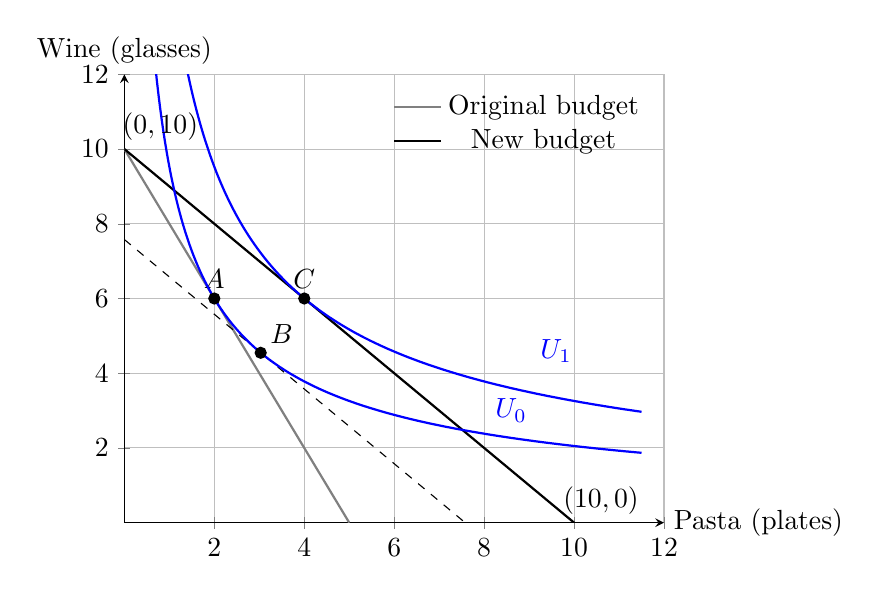
\begin{tikzpicture}
\begin{axis}[
    axis lines=middle,
    xlabel={Pasta (plates)},
    ylabel={Wine (glasses)},
    xmin=0, xmax=12,
    ymin=0, ymax=12,
    xtick={0,2,4,6,8,10,12},
    ytick={0,2,4,6,8,10,12},
    grid=both,
    legend style={at={(0.98,0.98)},anchor=north east, draw=none, fill=none},
    every axis x label/.style={at={(current axis.right of origin)}, anchor=west},
    every axis y label/.style={at={(current axis.above origin)}, anchor=south}
]

% ---------- Budget Lines ----------
% Original budget (p_pasta = 20, p_wine = 10): slope -2
\addplot[thick, gray] coordinates {(0,10) (5,0)};
\addlegendentry{Original budget}

% New budget (p_pasta = 10, p_wine = 10): slope -1
\addplot[thick, black] coordinates {(0,10) (10,0)};
\addlegendentry{New budget}

% ---------- Optima ----------
% A: Initial optimum (a=0.4 Cobb-Douglas) at (2,6)
\addplot[only marks, mark=*, mark size=2pt] coordinates {(2,6)};
\node[anchor=south] at (axis cs:2,6) {$A$};

% C: New optimum at (4,6)
\addplot[only marks, mark=*, mark size=2pt] coordinates {(4,6)};
\node[anchor=south] at (axis cs:4,6) {$C$};

% ---------- Hicks Compensated Point ----------
% B: Hicks substitution point where new price line (slope -1) is tangent to U0
% Computed (a=0.4): B ≈ (3.03, 4.55)
\addplot[only marks, mark=*, mark size=2pt] coordinates {(3.031,4.547)};
\node[anchor=south west] at (axis cs:3.031,4.547) {$B$};

% Compensated budget through B with slope -1: y = (y_B + x_B) - x
\addplot[dashed, domain=0:11.5, samples=2] {7.578 - x};

% ---------- Indifference Curves (Cobb–Douglas, a=0.4) ----------
% U0 through A=(2,6): y = C0 * x^{-2/3}, C0 = 6 * 2^{2/3} ≈ 9.5244
\addplot[thick, blue, domain=0.5:11.5, samples=300] {9.5244063118 * pow(x,-2/3)};
\node[blue] at (axis cs:8.6,3.0) {$U_0$};

% U1 through C=(4,6): y = C1 * x^{-2/3}, C1 = 6 * 4^{2/3} ≈ 15.1191
\addplot[thick, blue, domain=0.5:11.5, samples=300] {15.1190525987 * pow(x,-2/3)};
\node[blue] at (axis cs:9.6,4.6) {$U_1$};

% ---------- Intercepts Labels ----------
\node at (axis cs:0.8,10.6) {$(0,10)$};
\node at (axis cs:10.6,0.6) {$(10,0)$};

\end{axis}
\end{tikzpicture}






    
\end{enumerate}


\newpage
\section*{Question 3}
     Consider a firm which produces pizzas. The following table shows the number of pizzas produced given varying numbers of workers:
    
\begin{table}[H]
        \centering
        \begin{tabular}{cc}
            Workers & Output \\
            \hline
            0 & 0 \\
            1 & 20 \\
            2 & 45 \\
            3 & 80 \\
            4 & 100 \\
            5 & 110 \\
        \end{tabular}

        \label{tab:placeholder}
    \end{table}
    
     A worker costs \$100 and the firm has fixed costs of \$200. Add columns for the fixed cost, variable cost, total cost, average total cost, and marginal cost and fill them in.
    
\textbf{Answer:
}
\begin{table}[H]
        \centering
        \begin{tabular}{ccccccc}
            Workers & Output & Fixed Cost & Variable Cost & Total Cost & ATC & Marginal Cost \\
            \hline
            0 & 0 & 200 & 0 & 200 & - & -\\
            1 & 20 & 200 & 100 & 300 & 15 & 5 \\
            2 & 45 & 200 & 200 & 400 & 8.9 & 4\\
            3 & 80 & 200 & 300 & 500 & 6.25 & 2.86\\
            4 & 100 & 200 & 400 & 600 & 6 & 5\\
            5 & 110 & 200 & 500 & 700 & 6.36 & 10\\
        \end{tabular}

        \label{tab:placeholder}
    \end{table}

    And a corresponding graph to illustrate the relationship between MC and ATC:

    % In your preamble:
% \usepackage{pgfplots}
% \pgfplotsset{compat=1.18}

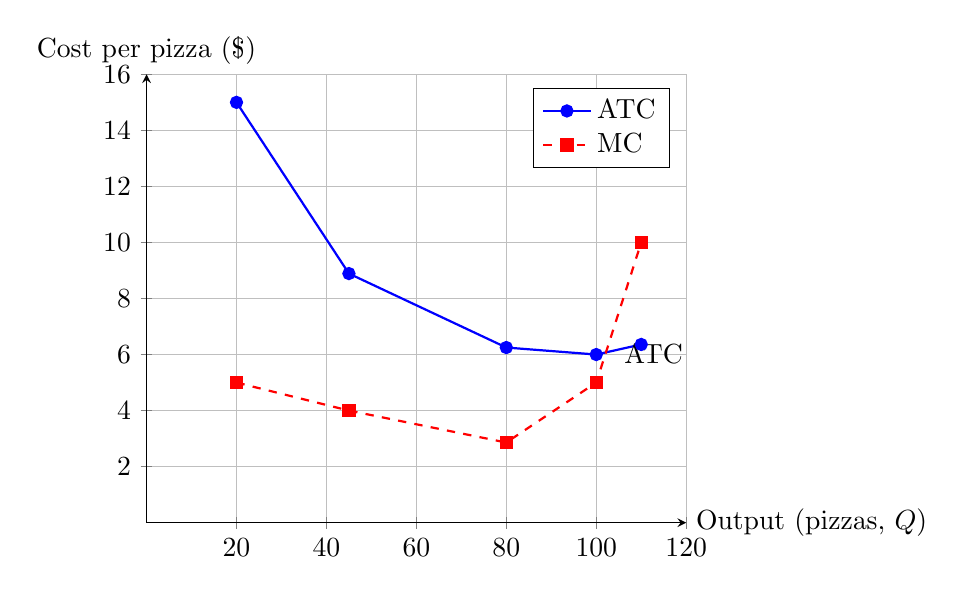
\begin{tikzpicture}
\begin{axis}[
  axis lines=middle,
  xlabel={Output (pizzas, $Q$)},
  ylabel={Cost per pizza (\$)},
  xmin=0, xmax=120,
  ymin=0, ymax=16,
  xtick={0,20,40,60,80,100,120},
  ytick={0,2,4,6,8,10,12,14,16},
  grid=both,
  legend pos=north east,
  legend cell align=left,
  every axis x label/.style={at={(current axis.right of origin)}, anchor=west},
  every axis y label/.style={at={(current axis.above origin)}, anchor=south}
]

% ATC points and connecting line
\addplot+[thick, mark=*, mark options={solid}]
  coordinates {(20,15.00) (45,8.89) (80,6.25) (100,6.00) (110,6.36)};
\addlegendentry{ATC}

% MC points and connecting line
\addplot+[thick, dashed, mark=square*, mark options={solid}]
  coordinates {(20,5.00) (45,4.00) (80,2.86) (100,5.00) (110,10.00)};
\addlegendentry{MC}

% (Optional) mark the ATC minimum at Q=100
\node[anchor=west] at (axis cs:100,6.0) {~~ATC min};

\end{axis}
\end{tikzpicture}

\end{document}
